%%%%%%%%%%%%%%%%%%%%%%%%%%%%%%%%%%%%%%%%%%%%%%%%%%%%%%%%%%%%%%%%%%%%%%%%%%%%%%%
% PREAMBOLO COMUNE PER APPUNTI (Stile Scuro)
%
% Questo file contiene tutte le impostazioni e i pacchetti comuni.
% NON contiene \begin{document} o \end{document}.
%
% Istruzioni per la compilazione del file principale:
% pdflatex -shell-escape nomefile_principale.tex
%%%%%%%%%%%%%%%%%%%%%%%%%%%%%%%%%%%%%%%%%%%%%%%%%%%%%%%%%%%%%%%%%%%%%%%%%%%%%%%

\documentclass{article}

% --- Encoding e lingua ---
\usepackage[utf8]{inputenc}
\usepackage[italian]{babel}

% --- Margini e layout ---
\usepackage{geometry}
\geometry{a4paper, margin=1in}

% --- Font sans-serif (come Helvetica) ---
\usepackage[scaled]{helvet}
\renewcommand{\familydefault}{\sfdefault}
\usepackage[T1]{fontenc}

% --- Matematica ---
\usepackage{amsmath}
\usepackage{amssymb}

% --- Liste personalizzate ---
\usepackage{enumitem}
% \setlist{nosep}

% --- Immagini e Grafica ---
\usepackage{float}
% \usepackage{graphicx}
\usepackage{tikz}
\usetikzlibrary{shapes.geometric, positioning, arrows.meta, calc, fit, backgrounds, patterns, decorations.pathreplacing}

% --- Tabelle Avanzate ---
\usepackage{array}
\usepackage{booktabs}
\usepackage{longtable}

% --- Hyperlink e Metadati PDF ---
\usepackage{hyperref}

\hypersetup{
    colorlinks=true,
    linkcolor=white,
    filecolor=magenta,
    urlcolor=cyan,
    citecolor=green,
    % pdftitle, pdfauthor, ecc. verranno impostati nel file principale
    pdfpagemode=FullScreen,
    bookmarksopen=true,
    bookmarksnumbered=true
}

% --- Licenza del documento ---
\usepackage[
  type={CC},
  modifier={by-sa},
  version={4.0},
]{doclicense}

% --- Colori e Sfondo Nero ---
\usepackage{xcolor}
\pagecolor{black}
\color{white}

% --- Evidenziazione del Codice ---
\usepackage{minted}
\setminted{
    frame=lines,
    framesep=2mm,
    fontsize=\small,
    breaklines=true,
    style=monokai,
    bgcolor=black!80
}
\usemintedstyle{monokai}

% --- Comandi personalizzati per algebra relazionale ---
\newcommand{\Rel}[1]{\textit{#1}} % Per i nomi delle relazioni
\newcommand{\Attr}[1]{\textsf{#1}} % Per i nomi degli attributi

\newcommand{\myunion}{\cup}
\newcommand{\myintersection}{\cap}
\newcommand{\mydifference}{-}
\newcommand{\myrename}[2]{\rho_{#1}(#2)}
\newcommand{\myselectop}[2]{\sigma_{#1}(#2)}
\newcommand{\myproject}[2]{\pi_{#1}(#2)}
\newcommand{\mycartesian}{\times}
\newcommand{\mynaturaljoin}{\bowtie} % Usare \Join da amssymb se disponibile e preferito
\newcommand{\mythetajoin}[3]{#1 \bowtie_{#2} #3} % R1 \bowtie_cond R2

% --- Comandi personalizzati per logica ---
\newcommand{\mylandop}{\wedge}
\newcommand{\myvel}{\vee}
\newcommand{\mynegop}{\neg}
\newcommand{\myforallop}{\forall}
\newcommand{\myexistsop}{\exists}

% --- Join esterni (outer join) ---
% Definizione standard per i join esterni
\def\ojoin{\setbox0=\hbox{$\mynaturaljoin$}%
	\rule[-.02ex]{.25em}{.4pt}\llap{\rule[\ht0]{.25em}{.4pt}}}
\newcommand{\myleftouterjoin}{\mathbin{\ojoin\mkern-5.8mu\mynaturaljoin}}
\newcommand{\myrightouterjoin}{\mathbin{\mynaturaljoin\mkern-5.8mu\ojoin}}
\newcommand{\myfullouterjoin}{\mathbin{\ojoin\mkern-5.8mu\mynaturaljoin\mkern-5.8mu\ojoin}}



% --- Titolo ---
\title{\textbf{Appunti sul Livello Applicazione}}
\author{Basato sulle slide del Corso di Reti di Calcolatori}
\date{\today}

% Stili TikZ
\tikzstyle{host} = [rectangle, rounded corners, draw=cyan, fill=blue!20, minimum height=2em, minimum width=3em, text=lighttext]
\tikzstyle{servernode} = [cylinder, shape border rotate=90, draw=orange, fill=orange!20, aspect=0.5, minimum height=2.5em, text=lighttext]
\tikzstyle{process} = [rectangle, draw=green, fill=green!10, minimum height=1.5em, text=lighttext]
\tikzstyle{cloud} = [ellipse, draw=gray, fill=gray!10, minimum height=3em, minimum width=5em, text=lighttext]
\tikzstyle{datagram} = [rectangle, draw=yellow, fill=yellow!10, minimum width=2.5cm, text=black, font=\small, align=center] % Aumentato da \tiny a \small
\tikzstyle{arrow} = [-{Stealth[length=3mm, width=2mm]}, thick, orange]
\tikzstyle{line} = [thick, gray!80]
\tikzstyle{r_arrow} = [{Stealth[length=3mm, width=2mm]}-, thick, orange] % Reversed arrow

% Comandi personalizzati per diagrammi
\tikzstyle{actor} = [rectangle, draw, fill=blue!20, text=white,
    minimum height=1cm, minimum width=2cm, text centered]
\tikzstyle{message_r} = [->, >=Stealth, thick]
\tikzstyle{message_l} = [<-, >=Stealth, thick]
\tikzstyle{channel} = [draw, thick, loosely dashed, blue!50]
\tikzstyle{intruder} = [star, star points=7, star point ratio=0.5, draw, fill=red!50, text=white, minimum size=1.5cm, text centered]
\tikzstyle{key} = [shape=key, shape border rotate=0, draw, fill=yellow!50, minimum size=0.5cm, font=\tiny]
\tikzstyle{dataflow} = [->, >=Stealth, thick, rounded corners]
\tikzstyle{block} = [rectangle, draw, fill=gray!20, text=white, minimum height=0.8cm, minimum width=2.5cm, text centered]
\tikzstyle{process} = [rectangle, draw, fill=green!20, text=white, rounded corners, minimum height=0.8cm, text centered]

\begin{document}

\maketitle
\tableofcontents
\newpage

\section{Principi delle Applicazioni di Rete}
L'obiettivo di questo capitolo è comprendere i concetti e gli aspetti implementativi dei protocolli di rete a livello applicazione, esaminare i protocolli più popolari (HTTP, FTP, SMTP, DNS) e capire come si creano applicazioni di rete usando le API socket.

\subsection{Architetture delle Applicazioni}
Esistono due strutture principali:

\begin{enumerate}
    \item \textbf{Client-Server:}
    \begin{itemize}
        \item \textbf{Server:}
        \begin{itemize}
            \item Host sempre attivo ("always-on").
            \item Indirizzo IP permanente.
            \item Spesso organizzato in data center per scalabilità.
        \end{itemize}
        \item \textbf{Client:}
        \begin{itemize}
            \item Comunicano con il server.
            \item Possono essere connessi in modo intermittente.
            \item Possono avere indirizzi IP dinamici.
            \item \textbf{Non} comunicano direttamente tra loro.
        \end{itemize}
        \item \textit{Esempio pratico:} Accesso email (PC client, server email Gmail).
    \end{itemize}

\begin{figure}[H]
    \centering
    \begin{tikzpicture}[node distance=2cm and 3cm,
        every node/.style={text=primarytext}]
        \node[servernode, label=below:Server] (server) {};
        \node[host, left=of server, label=below:Client 1] (client1) {};
        \node[host, above=of client1, label=below:Client 2] (client2) {};
        \node[host, right=of server, label=below:Client 3] (client3) {};

        \draw[arrow] (client1.east) -- (server.west) node[midway, above, sloped, font=\small]{Richiesta};
        \draw[r_arrow] (client1.east) -- (server.west) node[midway, below, sloped, font=\small]{Risposta};
        \draw[arrow] (client2.east) -- (server.west);
        \draw[arrow] (client3.west) -- (server.east);
    \end{tikzpicture}
    \caption{Architettura Client-Server.}
\end{figure}

    \item \textbf{Peer-to-Peer (P2P):}
    \begin{itemize}
        \item \textbf{Nessun server always-on} dedicato.
        \item Sistemi terminali arbitrari (peer) comunicano direttamente.
        \item \textbf{Auto-scalabilità:} Nuovi peer portano nuova capacità.
        \item Gestione più complessa a causa di connessioni intermittenti e IP dinamici.
        \item \textit{Esempio pratico:} BitTorrent.
    \end{itemize}
\begin{figure}[H]
    \centering
    \begin{tikzpicture}[node distance=1.5cm]
        \node[host, label=below:Peer A] (pA) {};
        \node[host, right=of pA, label=below:Peer B] (pB) {};
        \node[host, below=of pA, label=below:Peer C] (pC) {};
        \node[host, below=of pB, label=below:Peer D] (pD) {};

        \draw[arrow, <->] (pA.east) -- (pB.west);
        \draw[arrow, <->] (pA.south) -- (pC.north);
        \draw[arrow, <->] (pB.south) -- (pD.north);
        \draw[arrow, <->] (pC.east) -- (pD.west);
        \draw[arrow, <->] (pA.south east) -- (pD.north west);
    \end{tikzpicture}
    \caption{Architettura Peer-to-Peer.}
\end{figure}
\end{enumerate}


\subsection{Processi Comunicanti}
\begin{itemize}
    \item Un \textbf{processo} è un programma in esecuzione.
    \item Processi su host diversi comunicano scambiandosi \textbf{messaggi}.
    \item \textbf{Processo client:} Inizia la comunicazione.
    \item \textbf{Processo server:} Attende di essere contattato.
\end{itemize}

\subsection{Socket}
\begin{itemize}
    \item Un processo invia/riceve messaggi attraverso una \textbf{socket}.
    \item Analoga a una "porta": il processo si affida all'infrastruttura di trasporto per la consegna.
    \item Lo sviluppatore controlla il lato applicazione, il SO controlla il lato trasporto.
\end{itemize}

\begin{figure}[H]
\centering
\begin{tikzpicture}[node distance=1.5cm and 1cm]
    % Host Sinistro
    \node[host] (hostL) {\textcolor{black}{Host A}};
    \node[process, above=2cm of hostL.north] (appL) {\textcolor{black}{Applicazione A}};
    \node[rectangle, draw=blue, fill=blue!10, minimum width=2.5cm, minimum height=0.7cm, below=1cm of appL] (transportL) {\textcolor{black}{Trasporto}};
    \node[rectangle, draw=yellow, fill=yellow!20, minimum width=1.2cm, minimum height=0.5cm, text=black] at ($(appL.south)!0.5!(transportL.north)$) (socketL) {Socket};
    
    % Host Destro
    \node[host, right=4cm of hostL] (hostR) {\textcolor{black}{Host B}};
    \node[process, above=2cm of hostR.north] (appR) {\textcolor{black}{Applicazione B}};
    \node[rectangle, draw=blue, fill=blue!10, minimum width=2.5cm, minimum height=0.7cm, below=1cm of appR] (transportR) {\textcolor{black}{Trasporto}};
    \node[rectangle, draw=yellow, fill=yellow!20, minimum width=1.2cm, minimum height=0.5cm, text=black] at ($(appR.south)!0.5!(transportR.north)$) (socketR) {Socket};

    % Connessione
    \node[cloud, below right=2cm and 0.5cm of transportL, minimum width=3cm] (internet) {\textcolor{black}{Internet}};
    \draw[line] (transportL.east) -- (internet.west);
    \draw[line] (transportR.west) -- (internet.east);
    
    % Linee socket-applicazione
    \draw[line, red, dashed] (appL.south) -- (socketL.north);
    \draw[line, red, dashed] (appR.south) -- (socketR.north);
    \draw[line, red, dashed] (socketL.south) -- (transportL.north);
    \draw[line, red, dashed] (socketR.south) -- (transportR.north);

    \node[font=\tiny, red, above left=1cm and -0.3cm of socketL] {Controllato da App Dev};
    \node[font=\tiny, red, below left=1cm and -0.3cm of socketL] {Controllato da OS};
\end{tikzpicture}
\caption{Concetto di Socket tra due processi applicativi.}
\end{figure}

\subsection{Indirizzamento dei Processi}
\begin{itemize}
    \item Per ricevere messaggi, un processo necessita di un identificatore.
    \item L'indirizzo IP dell'host non è sufficiente (molti processi per host).
    \item L'identificatore include \textbf{indirizzo IP} e \textbf{numero di porta}.
    \item \textit{Esempi di porte note:} HTTP porta 80, Mail (SMTP) porta 25.
\end{itemize}

\subsection{Cosa Definisce un Protocollo a Livello Applicazione?}
\begin{enumerate}
    \item \textbf{Tipi di messaggi scambiati} (es. richiesta, risposta).
    \item \textbf{Sintassi dei messaggi} (campi e loro delineazione).
    \item \textbf{Semantica dei messaggi} (significato dei campi).
    \item \textbf{Regole} (quando/come inviare e rispondere).
\end{enumerate}
\begin{itemize}
    \item \textbf{Protocolli aperti:} Definiti in RFC, permettono interoperabilità (es. HTTP, SMTP).
    \item \textbf{Protocolli proprietari:} Specifici di un prodotto (es. Skype inizialmente).
\end{itemize}

\subsection{Servizi di Trasporto Necessari a un'Applicazione}
\begin{itemize}
    \item \textbf{Integrità dei dati:} Alcune app richiedono 100\% affidabilità (file transfer), altre tollerano perdite (audio streaming).
    \item \textbf{Throughput:} Alcune app richiedono un minimo (multimedia), altre sono elastiche (email).
    \item \textbf{Timing (ritardo):} Alcune app richiedono basso ritardo (giochi, telefonia IP).
    \item \textbf{Sicurezza:} Crittografia, integrità.
\end{itemize}

\subsection{Servizi dei Protocolli di Trasporto Internet}
\begin{table}[H]
\centering
\begin{tabular}{|p{0.45\textwidth}|p{0.45\textwidth}|}
\hline
\textbf{TCP (Transmission Control Protocol)} & \textbf{UDP (User Datagram Protocol)} \\
\hline
\begin{itemize}[leftmargin=*]
    \item Trasporto \textbf{affidabile}
    \item \textbf{Controllo di flusso} e \textbf{controllo della congestione}
    \item \textbf{Orientato alla connessione}
    \item NON fornisce:
    \begin{itemize}
        \item garanzie di timing
        \item throughput minimo
        \item sicurezza intrinseca
    \end{itemize}
\end{itemize}
&
\begin{itemize}[leftmargin=*]
    \item Trasferimento dati \textbf{non affidabile}
    \item NON fornisce:
    \begin{itemize}
        \item affidabilità
        \item controllo di flusso/congestione
        \item timing
        \item throughput
        \item sicurezza
        \item setup di connessione
    \end{itemize}
    \item \textit{Vantaggi:}
    \begin{itemize}
        \item Più veloce
        \item Più controllo all'applicazione
        \item No controllo congestione
        \item Utile per app che tollerano perdite
        \item Ideale per query-risposta veloci (es. DNS)
    \end{itemize}
\end{itemize} \\
\hline
\end{tabular}
\caption{Confronto tra TCP e UDP.}
\label{tab:tcp-vs-udp}
\end{table}

\subsection{Applicazioni Internet e Protocolli di Trasporto}
\begin{table}[H]
\centering
\begin{tabular}{|l|l|l|}
\hline
\textbf{Applicazione}     & \textbf{Protocollo Liv. App.} & \textbf{Protocollo Trasporto} \\ \hline
E-mail                 & SMTP [RFC 2821]           & TCP                           \\
Accesso terminale remoto & Telnet [RFC 854]          & TCP                           \\
Web                    & HTTP [RFC 2616]           & TCP                           \\
Trasferimento file     & FTP [RFC 959]             & TCP                           \\
Streaming multimedia   & HTTP (es. YouTube), RTP   & TCP o UDP                     \\
Telefonia Internet     & SIP, RTP, proprietari     & TCP o UDP                     \\ \hline
\end{tabular}
\caption{Applicazioni comuni e i loro protocolli di trasporto.}
\end{table}

\subsection{Securing TCP (Rendere TCP Sicuro)}
\begin{itemize}
    \item TCP/UDP base non offrono crittografia.
    \item \textbf{SSL/TLS (Secure Sockets Layer / Transport Layer Security):}
    \begin{itemize}
        \item Fornisce una connessione TCP crittografata.
        \item Garantisce integrità dei dati e autenticazione degli endpoint.
        \item SSL è a livello applicazione: le app usano librerie SSL che "parlano" con TCP.
    \end{itemize}
\end{itemize}

\section{Web e HTTP (HyperText Transfer Protocol)}
\subsection{Concetti base}
\begin{itemize}
    \item Una \textbf{pagina web} consiste di \textbf{oggetti} (file HTML, JPEG, etc.).
    \item Un file HTML base include riferimenti ad altri oggetti.
    \item Ogni oggetto è indirizzabile tramite un \textbf{URL (Uniform Resource Locator)}.
    \item Esempio URL: \url{http://www.someschool.edu/someDept/pic.gif}
    (\texttt{www.someschool.edu} = nome host, \texttt{/someDept/pic.gif} = nome percorso).
\end{itemize}

\subsection{Panoramica HTTP}
\begin{itemize}
    \item Protocollo client/server del Web.
    \item \textbf{Client:} Browser (richiede, riceve, visualizza).
    \item \textbf{Server:} Web server (invia oggetti).
    \item HTTP usa \textbf{TCP} (solitamente porta 80).
    \item HTTP è \textbf{"stateless"} (senza stato): il server non mantiene info sulle richieste passate.
\end{itemize}

\subsection{Connessioni HTTP}
\begin{description}
    \item[HTTP Non Persistente]\mbox{}\\
    \begin{itemize}
        \item Max un oggetto per connessione TCP. Connessione chiusa dopo.
        \item Oggetti multipli richiedono connessioni multiple.
        \item Tempo di risposta per un oggetto: $2 \times \text{RTT} + \text{tempo trasmissione file}$.
    \end{itemize}
\begin{figure}[H]
\centering
\begin{tikzpicture}[
    % Define consistent spacing parameters
    node distance=2cm,
    horiz_space/.style={minimum width=6cm},
    vert_step/.style={minimum height=1cm},
    % Define common arrow styles
    req_arrow/.style={arrow, thick},
    resp_arrow/.style={arrow, dashed, thick},
    >=Stealth
]
    % Define base coordinates for better positioning
    \coordinate (base_left) at (0,0);
    \coordinate (base_right) at (8,0);
    
    % Place main nodes with good spacing
    \node[host, label=left:Client] (client) at (base_left) {};
    \node[servernode, label=right:Server] (server) at (base_right) {};
    
    % RTT 1 - TCP Setup (with better spacing)
    \node[font=\small, text=primarytext] (rtt1_label) at ($(client.east)+(1.2,2)$) {RTT 1};
    \draw[req_arrow, themeblue] ($(client.east)+(0,2)$) -- node[above, font=\small, text=primarytext] 
        {1a. Richiesta TCP} ($(server.west)+(0,2)$);
    \draw[resp_arrow, themeblue] ($(client.east)+(0,1.4)$) -- node[above, font=\small, text=primarytext] 
        {1b. Ack TCP} ($(server.west)+(0,1.4)$);
    
    % RTT 2 - HTTP Exchange (well separated)
    \node[font=\small, text=primarytext] (rtt2_label) at ($(client.east)+(1.2,0.5)$) {RTT 2};
    \draw[req_arrow, red] ($(client.east)+(0,0.7)$) -- node[above, font=\small, text=primarytext] 
        {2. Richiesta HTTP} ($(server.west)+(0,0.7)$);
    \draw[resp_arrow, red] ($(client.east)+(0,0.1)$) -- node[above, font=\small, text=primarytext] 
        {3. Risposta HTTP} ($(server.west)+(0,0.1)$);
    
    % File Transmission (with clear separation)
    \draw[decoration={brace,amplitude=8pt}, decorate, thick, green!70!primarytext]
        ($(client.east)+(0,-1)$) -- node[below=8pt, font=\small, text=primarytext] 
        {Tempo Trasmissione File} ($(server.west)+(0,-1)$);
    
    % TCP Close (at bottom with good spacing)
    \draw[dotted, thick, themeblue] ($(client.east)+(0,-2)$) -- node[above, font=\small, text=primarytext] 
        {4. Chiusura TCP} ($(server.west)+(0,-2)$);

\end{tikzpicture}
\caption{Flusso di una richiesta HTTP Non Persistente (semplificato).}
\label{fig:http_non_persistent}
\end{figure}

    \item[HTTP Persistente]\mbox{}\\
    \begin{itemize}
        \item Oggetti multipli su una singola connessione TCP.
        \item Il server lascia la connessione aperta.
        \item Riduce RTT e overhead.
    \end{itemize}
\end{description}

\subsection{Messaggi HTTP}
Formato ASCII. Tipi: \texttt{request} e \texttt{response}.
\subsubsection{Messaggio di Richiesta HTTP}
\begin{minted}{text}
GET /index.html HTTP/1.1
Host: www-net.cs.umass.edu
User-Agent: Firefox/3.6.10
Accept: text/html,application/xhtml+xml
Connection: keep-alive

(Corpo del messaggio opzionale per POST)
\end{minted}
\begin{itemize}
    \item \textbf{Request line:} metodo, URL, versione.
    \item \textbf{Header lines:} coppie nome-valore.
    \item \textbf{Entity Body:} dati per POST/PUT.
\end{itemize}

\subsubsection{Metodi HTTP}
\begin{itemize}
    \item \textbf{HTTP/1.0:} \texttt{GET}, \texttt{POST}, \texttt{HEAD}.
    \item \textbf{HTTP/1.1 aggiunge:} \texttt{PUT}, \texttt{DELETE}.
    \item Upload form: \texttt{POST} (dati nel corpo), \texttt{GET} (dati nell'URL).
\end{itemize}

\subsubsection{Messaggio di Risposta HTTP}
\begin{minted}{text}
HTTP/1.1 200 OK
Date: Sun, 26 Sep 2010 20:09:20 GMT
Server: Apache/2.0.52 (CentOS)
Last-Modified: Tue, 30 Oct 2007 17:00:02 GMT
Content-Length: 2652
Content-Type: text/html; charset=ISO-8859-1

(Corpo del messaggio: oggetto richiesto)
\end{minted}
\begin{itemize}
    \item \textbf{Status line:} versione, codice stato, frase stato.
    \item \textbf{Header lines}.
    \item \textbf{Entity Body:} oggetto.
\end{itemize}

\subsubsection{Codici di Stato HTTP (esempi)}
\begin{itemize}
    \item \texttt{200 OK}: Successo.
    \item \texttt{301 Moved Permanently}: Oggetto spostato.
    \item \texttt{400 Bad Request}: Richiesta malformata.
    \item \texttt{404 Not Found}: Oggetto non trovato.
    \item \texttt{505 HTTP Version Not Supported}.
\end{itemize}

\subsection{Stato Utente-Server: Cookies}
HTTP è stateless. I cookies permettono di mantenere lo stato.
\begin{itemize}
    \item \textbf{Componenti:} Header \texttt{Set-Cookie} (server$\rightarrow$client), header \texttt{Cookie} (client$\rightarrow$server), file cookie sul client, database backend sul server.
    \item \textbf{Funzionamento:} Il server invia un ID cookie, il client lo salva e lo ripresenta nelle richieste successive. Il server usa l'ID per recuperare info utente.
    \item \textbf{Usi:} Autorizzazione, carrelli, raccomandazioni, sessioni.
\end{itemize}
\begin{figure}[H]
\centering
\includegraphics[width=\textwidth]{images/cookie_flow}
\caption{Cookie Interaction Flow Between Client and Server}
\end{figure}


\subsection{Web Caches (Proxy Server)}
\textbf{Obiettivo:} Soddisfare richieste client senza coinvolgere il server di origine.
\begin{itemize}
    \item Il browser invia richieste HTTP alla cache.
    \item Se l'oggetto è in cache, viene restituito. Altrimenti, la cache lo richiede all'origine, lo salva e lo restituisce.
    \item \textbf{Perché usarle?} Riduce tempo risposta, traffico su link accesso, aiuta distribuzione contenuti.
\end{itemize}
\begin{figure}[H]
\centering
\begin{tikzpicture}[node distance=2cm and 3cm]
    \node[host, label=below:Client 1] (client1) {};
    \node[host, label=below:Client 2, below=1cm of client1] (client2) {};
    \node[servernode, label=below:Proxy Cache, right=of $(client1)!0.5!(client2)$] (cache) {};
    \node[servernode, label=below:Origin Server, right=of cache] (origin) {};

    \draw[arrow] (client1.east) -- (cache.west |- client1.east) node[midway, above, font=\tiny]{Req};
    \draw[r_arrow] (client1.east) -- (cache.west |- client1.east) node[midway, below, font=\tiny]{Resp (da cache)};

    \draw[arrow] (client2.east) -- (cache.west |- client2.east) node[midway, above, font=\tiny]{Req};
    \draw[r_arrow, dashed, themeblue] (cache.east) -- (origin.west) node[midway, above, font=\tiny]{Req (cache miss)};
    \draw[arrow, dashed, themeblue] (cache.east) -- (origin.west) node[midway, below, font=\tiny]{Resp (da origine)};
    \draw[r_arrow] (client2.east) -- (cache.west |- client2.east) node[midway, below, font=\tiny]{Resp (da cache dopo fetch)};
\end{tikzpicture}
\caption{Funzionamento di una Web Cache.}
\end{figure}

\subsection{Conditional GET}
\textbf{Obiettivo:} Non inviare un oggetto se la cache ha una versione aggiornata.
\begin{itemize}
    \item Cache invia \texttt{If-Modified-Since: <data>} nella richiesta.
    \item Server risponde \texttt{304 Not Modified} (se aggiornato) o \texttt{200 OK} con oggetto (se obsoleto).
\end{itemize}

\section{Posta Elettronica (Electronic Mail)}
\subsection{Componenti principali}
\begin{enumerate}
    \item \textbf{User Agents (Agenti Utente):} Lettore di posta (Outlook, Thunderbird).
    \item \textbf{Mail Servers (Server di Posta):}
    \begin{itemize}
        \item \textbf{Mailbox:} Contiene messaggi in arrivo.
        \item \textbf{Message queue:} Contiene messaggi in uscita.
        \item \textbf{Protocollo SMTP:} Usato tra server di posta.
    \end{itemize}
    \item \textbf{SMTP (Simple Mail Transfer Protocol) [RFC 2821]:}
    \begin{itemize}
        \item Usa \textbf{TCP}, porta \textbf{25}.
        \item Trasferimento diretto server-mittente $\rightarrow$ server-ricevente.
        \item Fasi: Handshaking, Transfer, Closure.
        \item Interazione comando/risposta ASCII. Messaggi in ASCII 7-bit.
    \end{itemize}
\end{enumerate}

\subsection{Scenario: Alice invia un messaggio a Bob}
\begin{figure}[H]
\centering
\includegraphics[width=\textwidth]{images/email_flow}
\caption{Email Flow Between Alice and Bob}
\end{figure}

\subsection{Confronto SMTP vs HTTP}
\begin{itemize}
    \item HTTP: "pull", SMTP: "push".
    \item Entrambi: comando/risposta ASCII, codici stato.
    \item HTTP: un oggetto per risposta. SMTP: messaggi multipart.
\end{itemize}

\subsection{Formato del Messaggio Email (RFC 822)}
\begin{itemize}
    \item \textbf{Header lines:} \texttt{To:}, \texttt{From:}, \texttt{Subject:} (diversi da comandi SMTP).
    \item \textbf{Body:} Il messaggio (originariamente solo ASCII 7-bit; MIME per dati binari).
\end{itemize}

\subsection{Protocolli di Accesso alla Posta}
SMTP per consegna/memorizzazione; altri per recupero.
\begin{itemize}
    \item \textbf{POP3 (Post Office Protocol v3):} Autorizzazione, transazione (lista, recupera, cancella). Tipicamente "download and delete". Stateless.
    \item \textbf{IMAP (Internet Mail Access Protocol):} Messaggi sul server, organizzazione in cartelle, stateful.
    \item \textbf{HTTP:} Usato da webmail (Gmail, Hotmail).
\end{itemize}


\section{DNS (Domain Name System)}
\subsection{Scopo}
Tradurre nomi host leggibili (es. \url{www.google.com}) in indirizzi IP e viceversa.
\begin{itemize}
    \item Database \textbf{distribuito} gerarchico di \textbf{name server}.
    \item Protocollo a livello \textbf{applicazione} (usa UDP).
\end{itemize}

\subsection{Servizi DNS}
\begin{enumerate}
    \item Traduzione hostname $\rightarrow$ IP.
    \item Host aliasing (nomi canonici e alias).
    \item Mail server aliasing.
    \item Load distribution (più IP per un nome).
\end{enumerate}

\subsection{Perché non centralizzare DNS?}
Single point of failure, volume traffico, latenza, manutenzione. \textbf{Non scala!}

\subsection{DNS: Un Database Distribuito e Gerarchico}
\begin{figure}[H]
\centering
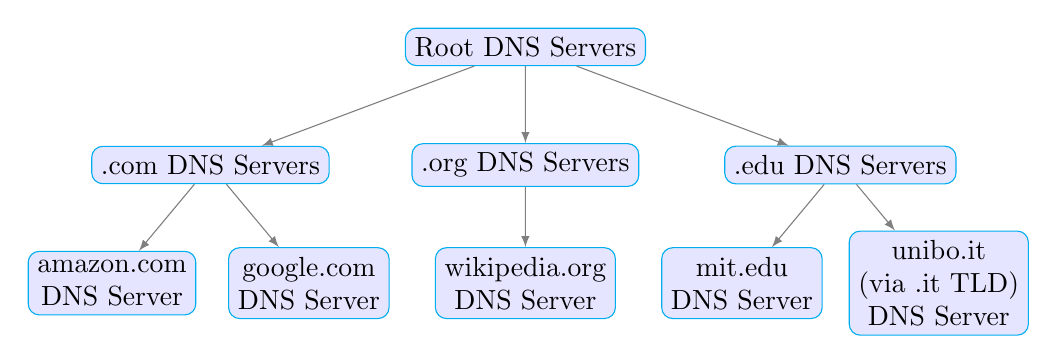
\begin{tikzpicture}[
    level 1/.style={sibling distance=4cm, level distance=1.5cm},
    level 2/.style={sibling distance=2.5cm, level distance=1.5cm},
    level 3/.style={sibling distance=1.5cm, level distance=1.5cm},
    edge from parent/.style={draw, -latex, gray},
    every node/.style={text=black},
    tnode/.style={rectangle, rounded corners, draw=cyan, fill=blue!10, text=black, align=center}
]
    \node[tnode] {Root DNS Servers}
    child { node[tnode] {.com DNS Servers}
        child { node[tnode] {amazon.com\\DNS Server} }
        child { node[tnode] {google.com\\DNS Server} }
    }
    child { node[tnode] {.org DNS Servers}
        child { node[tnode] {wikipedia.org\\DNS Server} }
    }
    child { node[tnode] {.edu DNS Servers}
        child { node[tnode] {mit.edu\\DNS Server} }
        child { node[tnode] {unibo.it\\(via .it TLD)\\DNS Server} }
    };
\end{tikzpicture}
\caption{Gerarchia semplificata dei server DNS.}
\end{figure}


\subsection{Local DNS Name Server}
\begin{itemize}
    \item Non strettamente nella gerarchia. Ogni ISP ne ha uno ("default name server").
    \item Query dell'host vanno qui. Ha cache locale. Agisce da proxy.
\end{itemize}

\subsection{Risoluzione Nomi DNS}
\begin{description}
    \item[Query Iterata:] Il server locale chiede in sequenza ai server radice, TLD, autoritativo. Ogni server risponde con il prossimo da contattare.
    \item[Query Ricorsiva:] Il carico della risoluzione è passato al server contattato. Spesso mix: ricorsiva client-locale, iterativa locale-gerarchia.
\end{description}
\begin{figure}[H]
\centering
\begin{tikzpicture}[node distance=1cm and 1.5cm, >=Stealth,
    tnode/.style={rectangle, rounded corners, draw=cyan, fill=blue!10, text=black, align=center, minimum height=1cm}]
    \node[host] (client) {\textcolor{black}{Client Host}};
    \node[tnode, right=of client, label=above:Local DNS] (local) {\textcolor{black}{Local DNS}};
    \node[tnode, above right=0.5cm and 1cm of local, label=above:Root DNS] (root) {\textcolor{black}{Root}};
    \node[tnode, right=of root, label=above:TLD DNS (.com)] (tld) {\textcolor{black}{TLD}};
    \node[tnode, below right=0.5cm and 1cm of tld, label=above:Authoritative DNS (example.com)] (auth) {\textcolor{black}{Authoritative}};

    \draw[arrow] (client.east) -- (local.west) node[midway, above, sloped, font=\tiny]{1. Query: www.example.com};
    \draw[arrow] (local.north east) -- (root.south west) node[midway, above, sloped, font=\tiny]{2. Query};
    \draw[r_arrow] (local.north east) -- (root.south west) node[midway, below, sloped, font=\tiny]{3. Resp: TLD addr};
    \draw[arrow] (local.east) -- (tld.west) node[midway, above, sloped, font=\tiny]{4. Query};
    \draw[r_arrow] (local.east) -- (tld.west) node[midway, below, sloped, font=\tiny]{5. Resp: Auth addr};
    \draw[arrow] (local.south east) -- (auth.north west) node[midway, above, sloped, font=\tiny]{6. Query};
    \draw[r_arrow] (local.south east) -- (auth.north west) node[midway, below, sloped, font=\tiny]{7. Resp: IP addr};
    \draw[r_arrow] (client.east) -- (local.west) node[midway, below, sloped, font=\tiny]{8. IP addr};
\end{tikzpicture}
\caption{Flusso di una query DNS Iterata (dal punto di vista del Local DNS).}
\end{figure}


\subsection{Caching DNS}
\begin{itemize}
    \item I name server mettono in cache le mappature apprese.
    \item Voci scadono dopo un TTL.
    \item Le voci in cache possono essere obsolete (DNS è "best effort").
\end{itemize}

\subsection{Record DNS (Resource Records - RR)}
Formato: \texttt{(name, value, type, ttl)}
\begin{itemize}
    \item \texttt{type=A}: Hostname $\rightarrow$ IPv4 address.
    \item \texttt{type=AAAA}: Hostname $\rightarrow$ IPv6 address.
    \item \texttt{type=NS}: Dominio $\rightarrow$ Hostname server DNS autoritativo.
    \item \texttt{type=CNAME}: Nome alias $\rightarrow$ Nome canonico.
    \item \texttt{type=MX}: Dominio $\rightarrow$ Nome mail server (+ priorità).
\end{itemize}

\subsection{Messaggi DNS}
Query e reply hanno stesso formato.
\begin{itemize}
    \item \textbf{Header:} Identification (ID query/reply), Flags (query/reply, ricorsione, etc.).
    \item \textbf{Sezioni:} Questions, Answers, Authority, Additional info.
\end{itemize}

\subsection{Inserimento di Record in DNS}
Es. Nuova startup "Network Utopia", \url{networkutopia.com}.
\begin{enumerate}
    \item Registra nome presso DNS registrar (es. GoDaddy).
    \begin{itemize}
        \item Fornisci IP dei tuoi server DNS autoritativi.
        \item Registrar inserisce RR (NS e A per il tuo server DNS) nel TLD server (\texttt{.com}).
    \end{itemize}
    \item Nel tuo server DNS autoritativo: crea record A per \url{www.networkutopia.com}, MX per \url{networkutopia.com}.
\end{enumerate}

\subsection{Attacchi DNS}
\begin{itemize}
    \item \textbf{DDoS attacks:} Bombardare server root/TLD.
    \item \textbf{Redirect attacks:} Man-in-the-middle, DNS poisoning.
    \item \textbf{Sfruttare DNS per DDoS (DNS Amplification):} Query piccole con IP sorgente falsificato $\rightarrow$ risposte grandi alla vittima.
\end{itemize}

\section{Applicazioni P2P (Peer-to-Peer)}
\begin{itemize}
    \item Nessun server always-on. Peer comunicano direttamente.
    \item Connessioni intermittenti, IP dinamici.
\end{itemize}

\subsection{Distribuzione File: Client-Server vs. P2P}
Tempo per distribuire file (dimensione $F$) a $N$ peer.
\begin{itemize}
    \item $u_s$: upload server. $d_i$: download peer $i$. $u_i$: upload peer $i$. $d_{min}$: min $d_i$.
    \item \textbf{Client-Server ($D_{c-s}$):} $D_{c-s} \ge \max\{N \cdot F/u_s, F/d_{min}\}$. Aumenta linearmente con $N$.
    \item \textbf{P2P ($D_{P2P}$):} $D_{P2P} \ge \max\{F/u_s, F/d_{min}, N \cdot F/(u_s + \sum u_i)\}$. Scala molto meglio.
\end{itemize}

\subsection{BitTorrent}
\begin{itemize}
    \item File diviso in \textbf{chunk}. Peer in un \textbf{torrent} scambiano chunk.
    \item \textbf{Tracker:} Server che traccia i peer.
    \item \textbf{Funzionamento:} Alice ottiene lista peer dal tracker, scambia chunk. Mentre scarica, carica.
    \item \textbf{Richiesta chunk:} "Rarest first" (i più rari prima).
    \item \textbf{Invio chunk (Tit-for-Tat):} Alice invia ai 4 peer che le inviano più velocemente. Unchoke ottimistico periodico.
\end{itemize}
\begin{figure}[H]
\centering
\begin{tikzpicture}[node distance=1.5cm, scale=0.8, transform shape]
    \node[servernode, label=above:Tracker] (tracker) {};
    \node[host, label=below:Peer1, below left=of tracker] (p1) {};
    \node[host, label=below:Peer2, below right=of tracker] (p2) {};
    \node[host, label=below:Peer3, right=of p2] (p3) {};
    \node[host, label=below:Peer4, below=of p1] (p4) {};
    \node[host, label=below:Peer5, below=of p2] (p5) {};
    
    \draw[arrow, dashed] (p1) -- (tracker);
    \draw[arrow, dashed] (p2) -- (tracker);
    \draw[arrow, dashed] (p3) -- (tracker);
    \draw[arrow, dashed] (p4) -- (tracker);
    \draw[arrow, dashed] (p5) -- (tracker);

    \draw[arrow, <->] (p1) -- (p2);
    \draw[arrow, <->] (p1) -- (p4);
    \draw[arrow, <->] (p2) -- (p3);
    \draw[arrow, <->] (p2) -- (p5);
    \draw[arrow, <->] (p4) -- (p5);
    \draw[arrow, <->, bend left] (p1) to (p5);
\end{tikzpicture}
\caption{Architettura semplificata di BitTorrent con Tracker e Peers.}
\end{figure}

\section{Video Streaming e CDN (Content Distribution Networks)}
\subsection{Contesto}
\begin{itemize}
    \item Traffico video è un grande consumatore di banda.
    \item \textbf{Sfide:} Scala (miliardi di utenti), Eterogeneità (capacità diverse).
    \item \textbf{Soluzione:} CDN.
\end{itemize}

\subsection{Multimedia: Video}
\begin{itemize}
    \item Sequenza di immagini (frame). Codifica usa ridondanza spaziale e temporale.
    \item \textbf{CBR (Constant Bit Rate):} Rate fisso.
    \item \textbf{VBR (Variable Bit Rate):} Rate variabile.
    \item Standard: MPEG-1, MPEG-2, MPEG-4.
\end{itemize}

\subsection{Streaming Multimedia: DASH (Dynamic, Adaptive Streaming over HTTP)}
\begin{itemize}
    \item \textbf{Server:} Video diviso in chunk, codificati a diverse velocità. \textbf{Manifest file} con URL dei chunk.
    \item \textbf{Client:} Misura banda, richiede chunk da manifest, sceglie rate max sostenibile. "Intelligenza" al client.
\end{itemize}

\subsection{Content Distribution Networks (CDN)}
\textbf{Sfida:} Streaming a molti utenti simultanei.
\begin{itemize}
    \item \textbf{Opzione 1 (Mega-server):} Non scala.
    \item \textbf{Opzione 2 (CDN):} Copie video su siti geograficamente distribuiti.
    \begin{itemize}
        \item \textbf{Enter deep:} Server CDN nelle reti di accesso (Akamai).
        \item \textbf{Bring home:} Cluster più grandi in POP vicini (Limelight).
    \end{itemize}
    \item \textbf{Funzionamento:} Utente diretto a copia vicina/performante. CDN operano "over the top" (OTT).
\end{itemize}
\begin{figure}[H]
\centering
\begin{tikzpicture}[node distance=1.5cm and 2cm, scale=0.9, transform shape]
    \node[servernode, label=above:Origin Server] (origin) {};
    
    \node[servernode, label=left:CDN Node A, below left=of origin] (cdnA) {\textcolor{black}{CDN A}};
    \node[servernode, label=right:CDN Node B, below right=of origin] (cdnB) {\textcolor{black}{CDN B}};
    \node[servernode, label=below:CDN Node C, below=2cm of origin] (cdnC) {CDN C};

    \node[host, label=left:User 1, below left=of cdnA] (user1) {};
    \node[host, label=right:User 2, below right=of cdnB] (user2) {};
    \node[host, label=below:User 3, below=of cdnC] (user3) {};
    \node[host, label=left:User 4, left=of cdnC] (user4) {};


    \draw[line, dashed, gray] (origin.south) -- (cdnA.north);
    \draw[line, dashed, gray] (origin.south) -- (cdnB.north);
    \draw[line, dashed, gray] (origin.south) -- (cdnC.north);

    \draw[arrow, green!50!black] (user1) -- (cdnA) node[midway, above, sloped, font=\tiny]{Request/Stream};
    \draw[arrow, green!50!black] (user2) -- (cdnB) node[midway, above, sloped, font=\tiny]{Request/Stream};
    \draw[arrow, green!50!black] (user3) -- (cdnC) node[midway, right, font=\tiny]{Req/Str};
    \draw[arrow, green!50!black] (user4) -- (cdnC) node[midway, left, font=\tiny]{Req/Str};

    \node[cloud, below=0.5cm of user3, minimum width=8cm, minimum height=1.5cm] (internet) {\textcolor{black}{Internet Backbone / Regional Networks}};
    \draw[line, gray!70] (cdnA) -- (internet.north -| cdnA);
    \draw[line, gray!70] (cdnB) -- (internet.north -| cdnB);
    \draw[line, gray!70] (cdnC) -- (internet.north);
\end{tikzpicture}
\caption{Concetto di Content Distribution Network (CDN).}
\end{figure}


\subsection{Accesso ai Contenuti CDN (Esempio)}
Bob richiede \url{http://netcinema.com/video}. Video su CDN KingCDN.
\begin{enumerate}
    \item Bob ottiene URL da \url{netcinema.com}.
    \item DNS per \url{netcinema.com} $\rightarrow$ il server DNS autoritativo di \url{netcinema.com} restituisce un URL che punta a KingCDN (es. \url{http://KingCDN.com/video_ID}).
    \item DNS per \url{KingCDN.com} $\rightarrow$ il server DNS autoritativo di KingCDN restituisce l'IP di un server CDN specifico, "migliore" per Bob.
    \item Bob fa streaming da quel server CDN.
\end{enumerate}

\subsection{Caso Studio: Netflix}
\begin{enumerate}
    \item Bob gestisce account.
    \item Sceglie video $\rightarrow$ Netflix (cloud Amazon) restituisce \textbf{manifest file} con URL chunk su server CDN.
    \item Client DASH fa streaming dai CDN. Netflix carica video (varie qualità) sui CDN.
\end{enumerate}

\section{Programmazione Socket}
\textbf{Obiettivo:} Costruire app client/server che comunicano via socket.
\textbf{Socket:} "Porta" tra processo applicativo e protocollo trasporto.

\subsection{Due tipi di socket}
\begin{itemize}
    \item \textbf{UDP:} Datagramma non affidabile, veloce.
    \item \textbf{TCP:} Byte-stream, affidabile, in ordine, lento.
\end{itemize}

\subsection{Esempio di Applicazione Semplice}
Client invia stringa, server la converte in maiuscolo, client la visualizza.

\subsection{Programmazione Socket con UDP}
\begin{itemize}
    \item No "connessione", no handshaking.
    \item Mittente allega IP dest + porta a ogni pacchetto. Ricevitore estrae IP mitt + porta.
    \item Dati persi/fuori ordine possibili.
\end{itemize}
\textbf{Interazione Socket UDP (concettuale):}
\begin{itemize}
    \item \textbf{Server:} \texttt{socket()} $\rightarrow$ \texttt{bind()} $\rightarrow$ loop: \texttt{recvfrom()} $\rightarrow$ processa $\rightarrow$ \texttt{sendto()}.
    \item \textbf{Client:} \texttt{socket()} $\rightarrow$ \texttt{sendto()} $\rightarrow$ \texttt{recvfrom()} $\rightarrow$ \texttt{close()}.
\end{itemize}
\begin{figure}[H]
\centering
\begin{tikzpicture}[node distance=1.5cm and 3cm]
    \node[process, label=above:Server (UDP), text=black] (server) {Server Process};
    \node[process, label=above:Client (UDP), text=black, right=of server] (client) {Client Process};

    \node[font=\small, below=0.1cm of server, align=center] (s1) {1. \texttt{socket(AF\_INET, SOCK\_DGRAM)}};
    \node[font=\small, below=0.3cm of s1, align=center] (s2) {2. \texttt{bind(port\_x)}};
    \node[font=\small, below=0.3cm of s2, align=center] (s3) {3. \texttt{recvfrom()} (attesa)};

    \node[font=\small, below=0.1cm of client, align=center] (c1) {1. \texttt{socket(AF\_INET, SOCK\_DGRAM)}};
    \node[font=\small, below=0.3cm of c1, align=center] (c2) {2. Prepara datagramma};
    \node[font=\small, below=0.3cm of c2, align=center] (c3) {3. \texttt{sendto(serverIP, port\_x)}};
    
    \draw[arrow, red] (c3.west) -- (s3.east) node[midway, above, font=\small]{Dati};
    
    \node[font=\small, below=0.3cm of s3, align=center] (s4) {4. Processa};
    \node[font=\small, below=0.3cm of s4, align=center] (s5) {5. \texttt{sendto(clientAddr)}};
    
    \node[font=\small, below=0.3cm of c3, align=center] (c4) {4. \texttt{recvfrom()} (attesa)};
    \node[font=\small, below=0.3cm of c4, align=center] (c5) {5. \texttt{close()}};
    
    \draw[r_arrow, themeblue] (c4.west) -- (s5.east) node[midway, above, font=\small]{Risposta};
\end{tikzpicture}
\caption{Interazione Socket UDP Client/Server (semplificata).}
\end{figure}

\subsection{Programmazione Socket con TCP}
\begin{itemize}
    \item Client contatta server. Server deve essere in esecuzione con socket di benvenuto (listening).
    \item Client: crea socket TCP, \texttt{connect()} $\rightarrow$ stabilisce connessione.
    \item Server: quando contattato, crea \textbf{nuova socket dedicata} (connection socket) per quel client.
    \item TCP fornisce byte-stream ("pipe") affidabile e in ordine.
\end{itemize}
\textbf{Interazione Socket TCP (concettuale):}
\begin{itemize}
    \item \textbf{Server:} \texttt{socket()} $\rightarrow$ \texttt{bind()} $\rightarrow$ \texttt{listen()} $\rightarrow$ loop: \texttt{accept()} (crea nuova socket) $\rightarrow$ comunica su nuova socket (\texttt{recv()}/\texttt{send()}) $\rightarrow$ \texttt{close()} (nuova socket).
    \item \textbf{Client:} \texttt{socket()} $\rightarrow$ \texttt{connect()} $\rightarrow$ comunica (\texttt{send()}/\texttt{recv()}) $\rightarrow$ \texttt{close()}.
\end{itemize}
\begin{figure}[H]
\centering
\begin{tikzpicture}[node distance=1.5cm and 4cm]
    \node[process, label=above:Server (TCP), text=black] (server) {Server Process};
    \node[process, label=above:Client (TCP), text=black, right=of server] (client) {Client Process};

    \node[font=\footnotesize, below=0.3cm of server, align=center] (s1) {1. \texttt{socket(SOCK\_STREAM)} (welcoming)};
    \node[font=\footnotesize, below=0.3cm of s1, align=center] (s2) {2. \texttt{bind(port\_x)}};
    \node[font=\footnotesize, below=0.3cm of s2, align=center] (s3) {3. \texttt{listen()}};
    \node[font=\footnotesize, below=0.3cm of s3, align=center] (s4) {4. \texttt{accept()} (attesa, crea connSocket)};

    \node[font=\footnotesize, below=0.3cm of client, align=center] (c1) {1. \texttt{socket(SOCK\_STREAM)}};
    \node[font=\footnotesize, below=0.3cm of c1, align=center] (c2) {2. \texttt{connect(serverIP, port\_x)}};
    
    \draw[arrow, <->, red] (c2.west) -- (s4.east) node[midway, above, font=\footnotesize, text=lighttext]{Handshake TCP};
    
    \node[font=\footnotesize, below=0.3cm of c2, align=center] (c3) {3. \texttt{send(data)}};
    \node[font=\footnotesize, below=0.3cm of s4, align=center] (s5) {5. \texttt{recv(data)} (su connSocket)};
    \draw[arrow, orange] (c3.west) -- (s5.east) node[midway, above, font=\footnotesize, text=lighttext]{Dati};

    \node[font=\footnotesize, below=0.3cm of s5, align=center] (s6) {6. Processa};
    \node[font=\footnotesize, below=0.3cm of s6, align=center] (s7) {7. \texttt{send(reply)} (su connSocket)};
    \node[font=\footnotesize, below=0.3cm of c3, align=center] (c4) {4. \texttt{recv(reply)}};
    \draw[r_arrow, themeblue] (c4.west) -- (s7.east) node[midway, above, font=\footnotesize, text=lighttext]{Risposta};
    
    \node[font=\footnotesize, below=0.3cm of s7, align=center] (s8) {8. \texttt{close(connSocket)}};
    \node[font=\footnotesize, below=0.3cm of c4, align=center] (c5) {5. \texttt{close()}};
\end{tikzpicture}
\caption{Interazione Socket TCP Client/Server (semplificata).}
\end{figure}


\subsection{Esempi Python (Concettuale)}
\subsubsection{UDPClient.py}
\begin{minted}{python}
from socket import *

serverName = 'hostname'
serverPort = 12000

# Crea un socket UDP
clientSocket = socket(AF_INET, SOCK_DGRAM)

# Ottieni input dall'utente
message = input('Input lowercase sentence:')

# Invia il messaggio al server
clientSocket.sendto(message.encode(), (serverName, serverPort))

# Ricevi la risposta dal server
modifiedMessage, serverAddress = clientSocket.recvfrom(2048)

# Stampa il messaggio ricevuto
print(modifiedMessage.decode())

# Chiudi il socket
clientSocket.close()
\end{minted}

\subsubsection{UDPServer.py}
\begin{minted}{python}
from socket import *
serverPort = 12000
serverSocket = socket(AF_INET, SOCK_DGRAM)
serverSocket.bind(('', serverPort))
print("The server is ready to receive")
while True:
    message, clientAddress = serverSocket.recvfrom(2048)
    modifiedMessage = message.decode().upper()
    serverSocket.sendto(modifiedMessage.encode(), clientAddress)
\end{minted}

\subsubsection{TCPClient.py}
\begin{minted}{python}
from socket import *
serverName = 'servername'
serverPort = 12000
clientSocket = socket(AF_INET, SOCK_STREAM)
clientSocket.connect((serverName,serverPort))
sentence = input('Input lowercase sentence:')
clientSocket.send(sentence.encode())
modifiedSentence = clientSocket.recv(1024)
print('From Server:', modifiedSentence.decode())
clientSocket.close()
\end{minted}

\subsubsection{TCPServer.py}
\begin{minted}{python}
from socket import *
serverPort = 12000
serverSocket = socket(AF_INET, SOCK_STREAM) # Welcoming socket
serverSocket.bind(('',serverPort))
serverSocket.listen(1)
print('The server is ready to receive')
while True:
    connectionSocket, addr = serverSocket.accept() # New socket for this client
    sentence = connectionSocket.recv(1024).decode()
    capitalizedSentence = sentence.upper()
    connectionSocket.send(capitalizedSentence.encode())
    connectionSocket.close() # Close connection socket, not welcoming socket
\end{minted}

\section{Recap}
\begin{itemize}
    \item \textbf{Architetture Applicative:} Client-server, P2P.
    \item \textbf{Requisiti Servizio Applicativo:} Affidabilità, banda, ritardo.
    \item \textbf{Modello Servizio Trasporto Internet:} TCP (affidabile, connessione), UDP (non affidabile, datagrammi).
    \item \textbf{Protocolli Specifici:} HTTP, SMTP/POP/IMAP, DNS, BitTorrent.
    \item \textbf{Video streaming, CDN.}
    \item \textbf{Programmazione Socket:} API per TCP e UDP.
\end{itemize}
\textbf{Temi Importanti Appresi sui Protocolli:}
\begin{itemize}
    \item Scambio messaggi richiesta/risposta.
    \item Formati messaggi (Headers, Data).
    \item Controllo vs. Messaggi (in-band, out-of-band).
    \item Centralizzato vs. Decentralizzato.
    \item Stateless vs. Stateful.
    \item Trasferimento affidabile vs. non affidabile.
    \item "Complessità ai margini della rete".
\end{itemize}

\section{NAT (Network Address Translation)}
\subsection{Concetto}
Permette a una rete locale di usare un solo IP pubblico.

\subsection{Motivazione per NAT}
\begin{itemize}
    \item Risparmio indirizzi IP pubblici.
    \item Flessibilità indirizzamento interno.
    \item Cambio ISP facile.
    \item Sicurezza parziale (dispositivi interni non direttamente indirizzabili).
\end{itemize}

\subsection{Implementazione}
Router NAT deve:
\begin{enumerate}
    \item \textbf{Datagrammi in Uscita:} Sostituire (IP sorg. locale, porta sorg. locale) con (IP NAT pub., nuova porta). Memorizzare traduzione in tabella NAT.
    \item \textbf{Datagrammi in Entrata:} Sostituire (IP dest. NAT pub., porta dest.) con (IP sorg. locale, porta sorg. locale) dalla tabella NAT.
\end{enumerate}

\subsection{Esempio Flusso NAT}

\begin{figure}[H]
    \centering
    \begin{tikzpicture}[scale=1.2]  % Reduced scale
        % Host, NAT, Server with reduced spacing
        \node[draw, rectangle, rounded corners, fill=blue!40!black, text=lighttext, minimum width=2.5cm, minimum height=1cm] (host) at (0,0) {Host 10.0.0.1};
        \node[draw, rectangle, fill=red!40!black, text=lighttext, minimum width=3cm, minimum height=1cm, align=center] (nat) at (4,0) {NAT Router\\(138.76.29.7)};  % Moved closer
        \node[draw, cylinder, fill=orange!40!black, text=lighttext, shape border rotate=90, aspect=0.3, minimum width=2.5cm, minimum height=2cm, align=center] (server) at (8,0) {Server\\128.119.40.186};  % Moved closer
        
        % NAT Table - more compact
        \node[draw, rectangle, text width=5cm, align=center, font=\small, fill=gray!30!black, text=lighttext] (table) at (4,-2.5) {  % Moved up
            \textbf{Tabella NAT}\\[0.1cm]
            138.76.29.7:5001 $\leftrightarrow$ 10.0.0.1:3345
        };
        
        % Connections with shorter labels
        \draw[->, thick, cyan] (host.east) -- (nat.west) 
            node[midway, above, font=\small, text=lighttext] {10.0.0.1:3345};
        \draw[->, thick, cyan] (nat.east) -- (server.west) 
            node[midway, above, font=\small, text=lighttext] {138.76.29.7:5001};
        \draw[<-, thick, orange] (host.east) -- (nat.west) 
            node[midway, below, font=\small, text=lighttext] {128...:80};
        \draw[<-, thick, orange] (nat.east) -- (server.west) 
            node[midway, below, font=\small, text=lighttext] {128...:80};
        
        % Table connection
        \draw[dashed, white, thick] (nat.south) -- (table.north);
    \end{tikzpicture}
    \caption{Esempio di flusso di un datagramma attraverso NAT.}
\end{figure}

\subsection{Considerazioni su NAT}
\begin{itemize}
    \item \textbf{Limitazione del Numero di Connessioni:}
    \begin{itemize}
        \item Il campo porta è di 16 bit $\rightarrow$ $2^{16} = 65.536$ porte totali
        \item Alcune porte sono riservate (0-1023)
        \item Quindi circa 60.000 connessioni simultanee possibili
        \item \textit{Esempio:} Se 100 dispositivi interni tentano di accedere ciascuno a 1000 servizi esterni, il NAT potrebbe esaurire le porte disponibili
    \end{itemize}
    
    \item \textbf{Controversie Architetturali:}
    \begin{itemize}
        \item Il router NAT modifica i pacchetti a livello trasporto (L4)
        \item Viola il principio end-to-end di Internet:
        \begin{center}
        \begin{tikzpicture}
            \node[host] (h1) at (0,0) {\textcolor{black}{Host A}};
            \node[draw=red, circle, fill=red!20] (nat) at (3,0) {\textcolor{black}{NAT}};
            \node[host] (h2) at (6,0) {\textcolor{black}{Host B}};
            
            \draw[->, thick, themeblue] (h1) -- node[above, yshift=0.4cm] {\small Dovrebbe essere diretto} (h2);
            \draw[->, thick, red, dashed] (h1) -- (nat);
            \draw[->, thick, red, dashed] (nat) -- (h2);
            \node[below, text width=6cm, align=center] at (3,-1) 
                {\small Il NAT interrompe la comunicazione diretta tra gli endpoint};
        \end{tikzpicture}
        \end{center}
        \item NAT è nato come soluzione temporanea alla carenza di IPv4
        \item La vera soluzione sarebbe la migrazione a IPv6 ($2^{128}$ indirizzi)
    \end{itemize}
    
    \item \textbf{Problemi con Applicazioni P2P:}
    \begin{itemize}
        \item In P2P, ogni peer dovrebbe poter accettare connessioni in ingresso
        \item Con NAT, i peer interni non sono direttamente raggiungibili dall'esterno
        \item \textbf{NAT traversal} necessario:
        \begin{center}
        \begin{tikzpicture}
            \node[host, label=below:Peer A] (p1) at (0,0) {};
            \node[draw=red, circle, fill=red!20, label=below:NAT] (nat) at (3,0) {};
            \node[host, label=below:Peer B] (p2) at (6,0) {};
            
            \draw[->, thick, red] (p2) -- node[above, yshift=0.3cm] {\small Bloccato dal NAT} (p1);
            \node[below, text width=8cm, align=center] at (3,-2) 
                {\small Soluzioni: STUN, TURN, ICE\\
                (protocolli per permettere la connessione attraverso NAT)};
        \end{tikzpicture}
        \end{center}
    \end{itemize}
\end{itemize}

\end{document}